\chapter{Notes}


\parencite{Merli2018} scholars approaching to circular economy concept


\begin{figure}[h!]
    \centering
    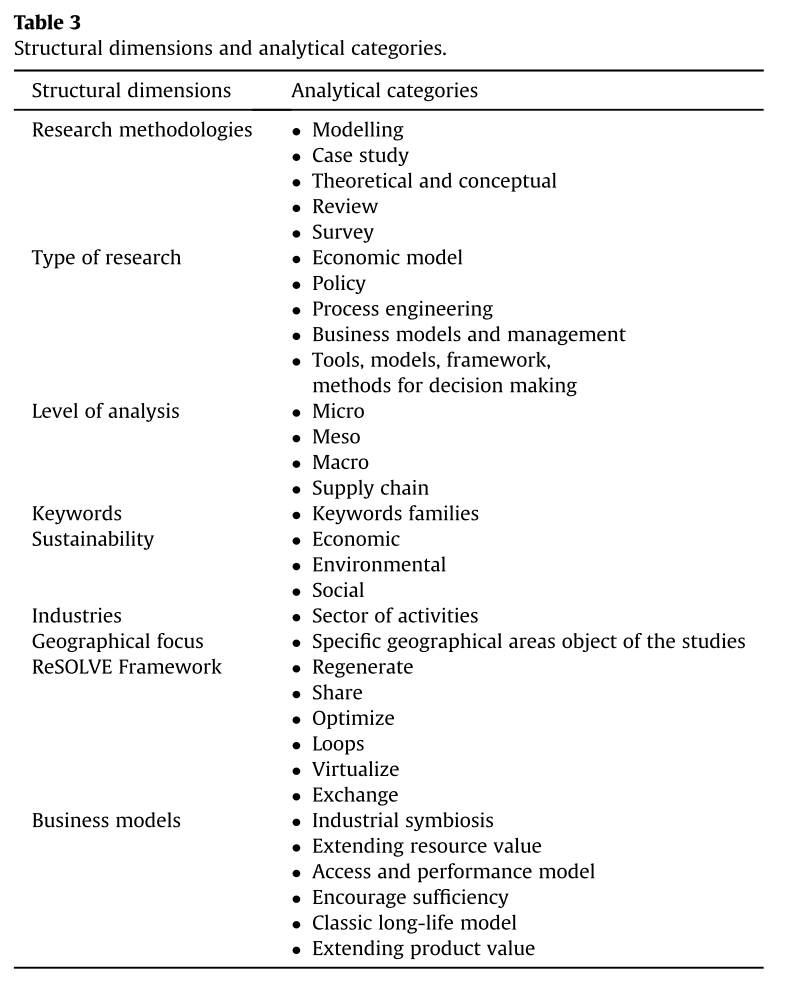
\includegraphics[width=0.8\textwidth]{sections/asset/cateogories of research.PNG}
    \caption{Cateogories of research}
    \label{fig:research cat}
\end{figure}


\subsection{Sustainability as contested}


\parencite{Stimson2006}


\begin{figure}[h!]
    \centering
    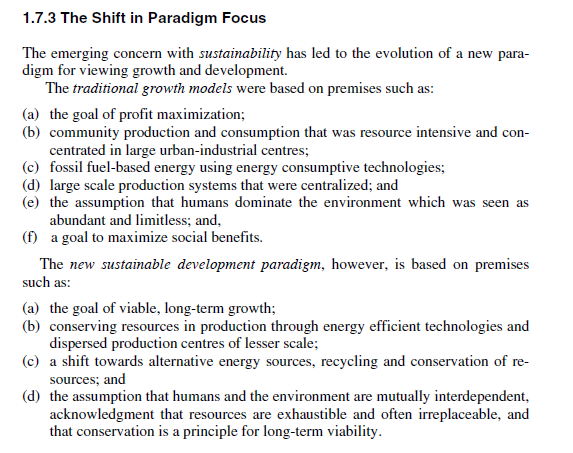
\includegraphics[width=0.8\textwidth]{sections/asset/shift.PNG}
    \caption{Change in paradigms}
    \label{fig:shift}
\end{figure}

Also on GIS

It is necessary to say something briefly about DSS in general. The goal of DSS is to focus ill-structured problems. As Densham (1994, p. 207) notes, DSSs are important when decision-makers “find it hard to define…problems and to articulate characteristics that they would like to see in a solution”. He argues that attributes of DSS include:\par
(a) support for the identification and use of data;\par
(b) the ability to represent complex relations among data which are needed for search, modelling and visualization;\par
(c) an architecture that is flexible enough to enable the user to combine model- ling and data in a variety of ways;\par
(d) an ability to generate a variety of types of output;\par
(e) a single, integrated, user interface which supports a variety of decision making styles; and\par
(f) an architecture that supports the addition of new capabilities as user needs evolve.




The new paradigm suggests that

This emerging new paradigm for regional economic development favours regions that have the human capital and technologies necessary to generate new knowledge and information—and to competently reinvent it—that creates the strategic architecture to facilitate a services dominated economy. The new paradigm will force regions to closely examine:
(a) what factors give them competitiveness? and \par
(b) how they may combine resources, competencies, assets, human capital and knowledge to become more efficient to create environments favourable for new economic development opportunities?\par
This paradigm assumes added significance when linked to another new paradigm being driven from an agenda that relates to ecological and resource capacity to support human populations and greater demands for economic equity. This is one of the great issues facing governments and communities throughout the world, including regional economies in the future. How we ensure economic development is more sustainable and equitable without forfeiting competitive advantage is uncertain and represents a significant challenge in formulating regional development strategies and for implementing plans.\par

During the 1990s, thinking on the new paradigm based on the concept of collaborative advantage (Huxham 1996) has advanced considerably, based on the prem- ise that networks, alliances, and partnerships are the replacing the more interventionalist strategies of the past, and these changes in strategic thinking (Hamel 1996; Mintzberg and Quinn 1992) are becoming more important and are being more fully incorporated in regional economic development strategy under con- temporary conditions of globalization, fast and flexible change. Strategy itself is also undergoing a major transformation, with a clearer separation of planning from strategy (Mintzberg 1994). As discussed in Chap. 5, strategy is now more the framework that provides a path for development and a direction for planning; it precedes planning. Planning is now being seen more as the instruments providing the mechanism for strategy implementation. Future regional economic development strategy will likely have three important functions. These are to:
(a) Identify key elements of capacity building to support economic development– the key elements of capacity building are what termed the strategic architecture of a region. \par
(b) Define strategic intent, in terms of the direction, destiny and discovery of opportunities for economic development in a region. \par
(c) Define the main thrusts of strategies for achieving strategic intent for managing economic development processes and for capacity building in a region—setting a future path. \par
The role of planning is to provide the details of initiatives, actions, resources, management, timing and delivery of resources, infrastructure, competencies and other supporting structures to execute strategy. Strategy is thus continuous and dynamic, while planning is more methodical and applied to the achievement of specific projects and outcomes.


The strategic architecture Hamel and Prahalad (1994) - \par
Much of the strategic architecture that can support the economic development of regions in the future similarly will be invisible or intangible. In the past, the strategic architecture of regional economies where their development was driven by comparative advantage, were strong in physical, financial and geographic terms. However, the strategic architecture required for regions to be successful in the ‘new’ economy of the contemporary global era is more in the form of technology, knowledge base and the virtual. Much greater knowledge is required about how to create that strategic architecture. This is where new tools for strategic planning—like multi-sectoral analysis (MSA) discussed in Chap. 7—can play a useful role in helping to develop strategic architecture by identifying:\par
(a) what competencies a region needs to build or maintain;\par
(b) what sector markets a region needs to develop or maintain;\par
(c) what strategic infrastructure to develop; \par
(d) what endowed resources to conserve and manage; and \par
(e) what approach to take to developing marketing intelligence.\par

The Challenge of the Virtual Economy
The development of communication technologies which enable organizations, institutions, and individuals to operate and manage activities in virtual space and communicate in virtual reality is changing significantly the conduct of business, social and economic transactions. The impact of the virtual economy may not be as profound as some writers would have us believe. It will, however, likely necessitate rewriting the rulebook of economic development practice. The virtual economy is the product of the information age. It is difficult to describe or define, but it is multi-dimensional and many of its elements are digital. There are many components of the virtual economy. These include:\par
(a) Organizations acting as brokers or catalysts for out-sourcing, coordinating, exchanging or disseminating goods and services using mainly telecommunications.\par
(b) The use of networks and alliances for business and other purposes. (c) Virtual simulation of events or experiences for recreational, commercial or re- search purposes and face to face video conferencing between people for consultation, inquiry, education and learning.\par
Almost every part of society in the developed world is being touched by the virtual economy and increasingly will be in the near future, as will also become the case in the developing regions.\par


\subsection{Urban and regional Planning}
\parencite{Friedmann1993}
'But what we are living through in the final decades of this century (1993) is something altogether different. It is nothing less than the collapse of the Euclidean world order of stable entities and common sense assumptions that have governed our understanding of the world for the past two hundred years.'
'We are moving into a non-Euclidean world of many space-time geographies, and it is the recognition of this change that obliges us to think of new and more appropriate models.'\par

[DEFINITION OF PLANNING]:
Planning is that professional practice that specifically seeks to connect forms of knowledge with forms of action in the public domain.'\par

'(...) we need first to consider the implications of the contemporary collapse of the time-space continuum. What would be the appropriate time and space of a non-Euclidean form of planning? The time of such planning is the \textit{real time} of everyday events rather than imagined future time.'\par

'Viewed in this light, planning becomes less a way of preparing documents, such as analyses and plans, and more a way of bridging planning knowledge and practice to bear directly on the action itself.'\par

'Concern with an imagined future will continue to play an important role in planning, but the emphasis in non-Euclidean planning should be on processes operating in actual or real time, because it is only in the evanescent and still undecided present that planners can hope to be effective.'\par

'As for the space of planning, we need to privilege \textit{regional and local} over national and transnational planning. This leads to a decentered view of planning 
-> 1. Heterogeneity of local places \par
-> 2. Organized civil society \par
-> 3. Regions and localities are the spaces of people's everyday lives. National and transnational space is typically for corporate actions and super ordinate bureaucracies.\par






\parencite{Casella2007}
'I have no quarrel with Friedmann’s characterization
of the non-Euclidian planning model as normative, innovative, political, transactive, and based on social learning. Those characteristics are validated by my own experience. But, I would add four other characteristics to Friedmann’s five, and call it a quantum model. A quantum planning model would also be technological, multidisciplinary, substantive, and intellectually free:'
description...



\parencite{WongTai-Chee;YuenBelinda;Goldblum2008}


Indeed, the concern with sustainable urban development arises and takes place in a world of economic globalization and of technological revolution, a world where the financial market’s selective expansion and innovation in the realm of communications systems has benefited strategic urban locations specifically catalytic to economic growth. Cities having built up a silent but revolutionary capacity in mastering flows (goods, people and information), in terms of paths and speed could affect their position and functions, their scale and ability in coping with these issues. If the rise of ecological ideas and consciousness in the early 1970s has been associated with “zero economic growth” (a concept promoted by the Club of Rome during the first oil crisis) and with the ideals of small/local dimensions (Schumacher 1973), the relationship between global dynamics and local development as expressed by the notion of “glocalism” are associated with mega-urban dimensions. The processes leading to this new representation of urban growth, the way to master its effects at urban, territorial and world scales, and to match it with the ideal of “sustainable development” naturally question the significance and the very nature of urban planning.\par

The objective of spatial planning for sustainability is primarily to counter the adverse effects of urban developments by means of systematic and organized land use planning activities. Sustainability planning has a holistic outlook which calls for an integration of the goals of the three Es (Economic, Environmental and Equity concerns) into an organized coherent system for a long-term objective formulation and plan implementation. No country can or should conduct sustainability planning in isolation, as the “stretching and deepening of global-scale processes” has exerted intricate interaction and reaction in one way or another on local scales (see Olds 2001: 19).\par



In terms of objectives, planning was no more dedicated to solving urban problems (in the sense of a corrective urbanism), but as a way to rationalize the city machinery itself, and to make it an efficient engine for nation-building and economic development.  










\subsection{Circular Economy}


About the concept \parencite{Prieto-Sandoval2018}



\parencite{Yuan2006}

\begin{figure}[h!]
    \centering
    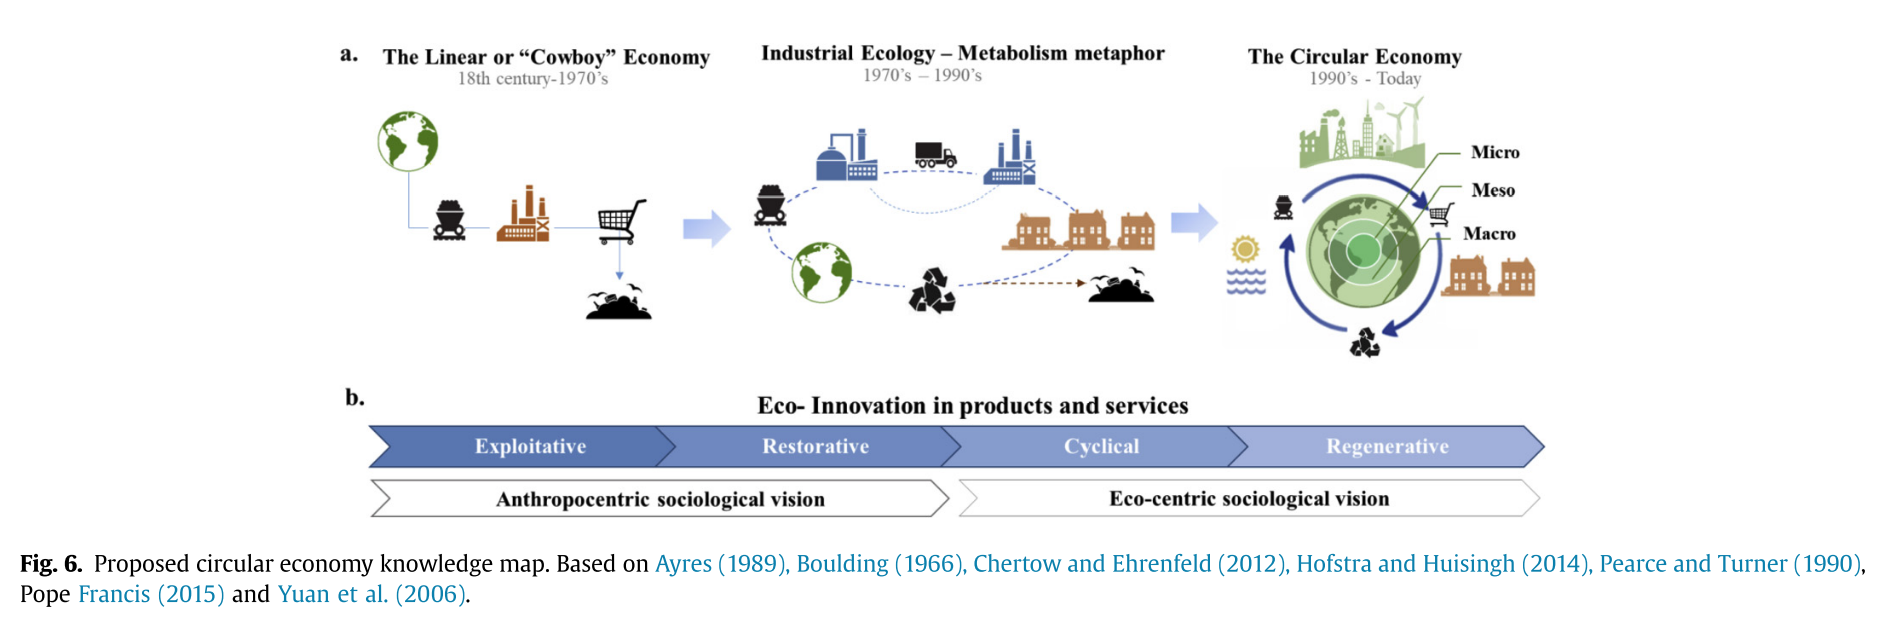
\includegraphics[width=0.8\textwidth]{sections/asset/model_strips.PNG}
    \caption{Models of economy}
    \label{fig:econ_models}
\end{figure}



\parencite{Gregson2015}
The concept of the circular economy has gained increasing prominence in academic, practitioner and policy circles and is linked to greening economies and sustainable development. However, the idea is more often celebrated than critically interrogated. Analysis shows the concept circulates as an idea and ideal, exemplified by industrial symbiosis and extended product life. Yet, its actual enactment is limited and fragile. Instead, circular economies are achieved mostly through global recycling networks which are the primary means by which wastes are recovered as resources. European policies eschew these circuits. Resource recovery through global recycling networks is regarded as a dirty and illegal trade. In its place, EU circular economies attempt to transform wastes into resources within the boundaries of the EU. Through an analysis of two case studies of resource recovery in the United Kingdom, we highlight the challenges that confront making circular economies within the EU, showing that these are borne of a conjuncture of politically created markets, material properties and morally defined materials circuits. We show resource recovery in the EU to be framed by moral economies, driven by discourses of ecological modernization environmental justice and resource (in)security, the last of which connects to China’s resource-intensive development.

This paper has subjected the concept of the circular economy to critical interrogation, by examining its instantiation in real world economies. The concept is an endlessly recited ideal. Yet, to effect a circular economy driven by producers through either industrial symbiosis or cradle-to-cradle manufacturing would require radical transformations to the economic order, including fundamental recasting of manufacture, retail, consumption and property rights. Beyond the ideal, in the messy world of how circularity is being enacted in actual economies, post-consumer wastes have become the basis for circular economies. One way in which this occurs is through global recycling networks, and new research has done much to make these activities visible. However, they do not count as appropriate forms of resource recovery and recycling in EU policies, where they are regarded as deeply suspect. Instead, under the rubric ‘high-quality recycling’, policy aims for the transformation of waste to resource within the EU. \par 


The question that remains is what form of politics lies behind this increasingly moral European market in resource recovery. There are three answers to this question. The first is a technocratic politics.
One element to this rests in the EU’s condemning of landfill.The underlying premise of this technocratic politics, however, is the technical dream of the perfect circle achieved via perfect recovery. This is technologic- ally impossible, as is illustrated by both dry recyclables and anaerobic digestion, both of which, whilst they recycle, also generate troublesome wastes as remainders of processing, and which continue to rely on landfill and/or incineration for their disposal. The second form of politics is environmental, driven by environmental
justice concerns. In continuing to portray global recycling as the global dumping of wastes on the people and environments of the Global South by the consumers and businesses of the Global North, accounts imply that global circuits of materials break the circular economy.

The third form of politics framing the morality of the EU’s circular economies is located in the political economy of resources and particularly resource security. For the most part, this politics is articulated in terms of the degree to which EU resource demand can be met through secondary resources. Answers range from around 50 per cent with respect to certain materials, such as paper and iron and steel, but much less for many others, even with a technically impossible 100 per cent recovery rate, and there are some 14 raw materials, mostly metals, which feature on the ‘high’ supply risk list for the EU economies. These are metals critical to high-value EU-based manufacturing, including in the aerospace, automotive and communications sectors. The figure that haunts these discussions though is China, and its resource-intensive form of development, particularly fears that it is securing control of resources from Africa. Indeed, the vulnerability of important sectors of EU manufacturing to Chinese resource use has been demonstrated recently through China’s dramatic cut-backs in rare earth metal exports. With China accounting for 95 per cent of global rare earth supply, the 30 per cent export reduction of 2010 led to rapid price hikes and a much-publicized rare earth panic in the United States, EU and Japan.






The concept and research is at an infant stage and the lack of a proper operational definition makes it and Essentially Contested Concept \parencite{Korhonen2018}. 

'However, the CE approach has almost exclusively been developed and led by practitioners, i.e., policy-makers and business development agencies such as business consultants, business associations, business foundations etc. (e.g., EMAF, 2013; COM, 2014; CIRAIG, 2015). From a scholarly position, the conceptual discussions on CE are still in their infancy and the literature is only emerging.'

After the review, a proposal of the definition is made.

'CE is a sustainable development initiative with the objective of reducing the societal production-consumption systems' linear material and energy throughput flows by applying materials cycles, renewable and cascade-type energy flows to the linear system. CE promotes high value material cycles alongside more traditional recycling and develops systems approaches to the cooperation of producers, consumers and other societal actors in sustainable development work.' 


Circular Economy is not yet a new paradigm, mainly because is still not embedded in every day life. 

As a consequence of identifying CE as a cluster concept it is vital that future research is careful with the framing of its studies. We have, in particular, identified the unit of analysis as a critical aspect of capturing CE research, since CE can have a very wide span both in terms of research topics and the scope of the study 

We propose a model for categorization that supports CE researchers in differentiating between different research streams and foci (see Fig. 2). Through better framing of the research it will also be easier to evaluate the quality of the research

\parencite{CDR2005}


\begin{figure}[h!]
    \centering
    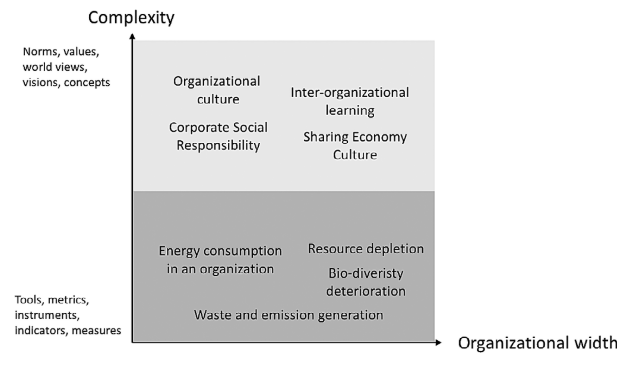
\includegraphics[width=0.8\textwidth]{sections/asset/stages_in_ce.PNG}
    \caption{Conceptual framework for CE research}
    \label{fig:stages}
\end{figure}


Using the umbrella concept in \textcite{Blomsma2017} conclude that whereas the various resource strategies grouped under the CE’s banner are not new individually, the concept offers a new framing of these strategies by drawing attention to their capacity of prolonging resource use as well as to the relationship between these strategies. As such, the CE offers a new perspective on waste and resource management and provides a new cognitive unit and discursive space for debate. 
Hirsch and Levin (1999) define an umbrella concept as: “a broad concept or idea used loosely to encompass and account for a set of diverse phenomena” (Hirsch and Levin (1999), 200). Umbrella concepts create a relation between pre-existing concepts that were previously unrelated, or not related in the manner the umbrella concept proposes, by focusing the attention on a particular shared quality or characteristic of the concepts it encompasses.


\begin{figure}[h!]
    \centering
    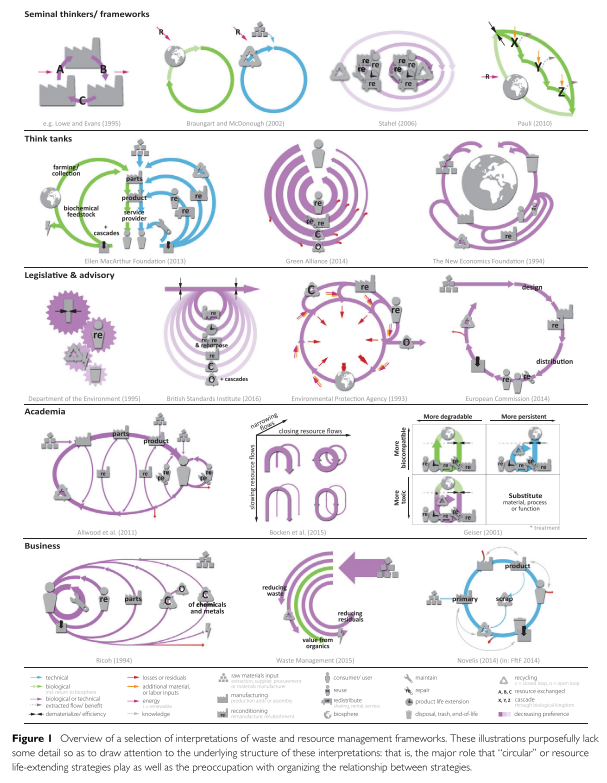
\includegraphics[width=0.8\textwidth]{sections/asset/ce_frameworks.PNG}
    \caption{Circular Economy frameworks}
    \label{fig:ce_frameworks}
\end{figure}

First, umbrella concepts typically arise when a field or discipline lacks guiding theories or a development paradigm.
Second, umbrella concepts typically progress along a predictable trajectory. This trajectory starts with the articulation of the umbrella concept by grouping pre-existing concepts. This phase is characterized by excitement and enthusiasm as the concept seemingly resolves the problem of too many unconnected concepts by providing a new framing that binds them together. After this phase, an umbrella concept usually sees its validity challenged when attempts at operationalizing the concept bring to the surface unresolved issues regarding its definition and assessment. A plurality of definitions, a lack of tools, and the existence of different indicators surface during this stage, raising questions regarding the nature of the binding capacity of the umbrella concept. This

\begin{figure}[h!]
    \centering
    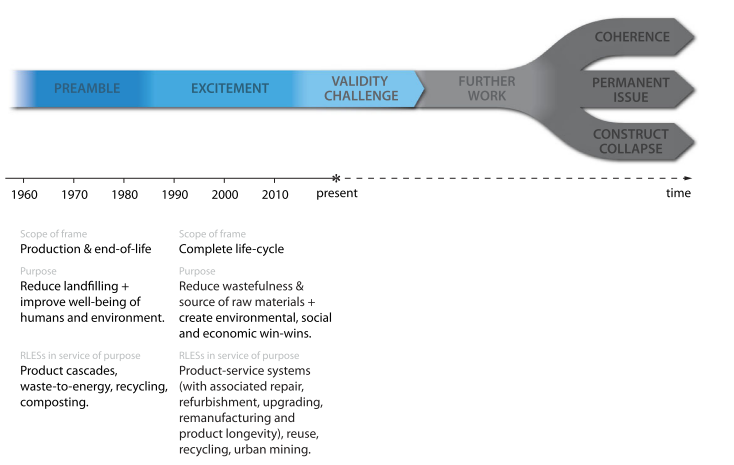
\includegraphics[width=0.8\textwidth]{sections/asset/ce_fork.PNG}
    \caption{Circular Economy trajectory}
    \label{fig:ce_trajectory}
\end{figure}


We are in the phase were the validity of the concept is being challenged. For instance, \parencite{Gregson2015,Gregson2015,Murray2017}, argue whether current interpretations are indeed in line with the creation of both societal and environmental benefits.

Not only quantitative work is needed. In order to make a socio-technical transformation other non-engineering questions need to be addressed. 

That is: Whereas answers to technical and engineering what questions are needed, which IE has traditionally engaged, what is also required if CE strategies are to be implemented are answers to how questions regarding accomplishing socioinstitutional change


\textcite{Korhonen2018a} However, the concept of CE and its practice have almost exclusively been developed and led by practitioners, i.e., policy-makers, businesses, business consultants, business associations, business foundations etc. (see e.g. EMAF, 2013; COM, 2014; CIRAIG, 2015). The scientific research content of CE remains largely unexplored. Ecological economics may be the most fruitful source from which the new practical, policy and business orientated concept of CE could find scientific and theoretical sup- port and guidance. Ecological economics has a long tradition in recycling and other CE-type concepts on the macroeconomic level al- though not presented under the CE term. Also on the microeconomic level, CE-type papers have been published in ecological economics



\textcite{Levoso2019} propose a methodology to implement CE in urban areas. This is based on the analysis of specific case studies on urban implementations.

\begin{figure}[h!]
    \centering
    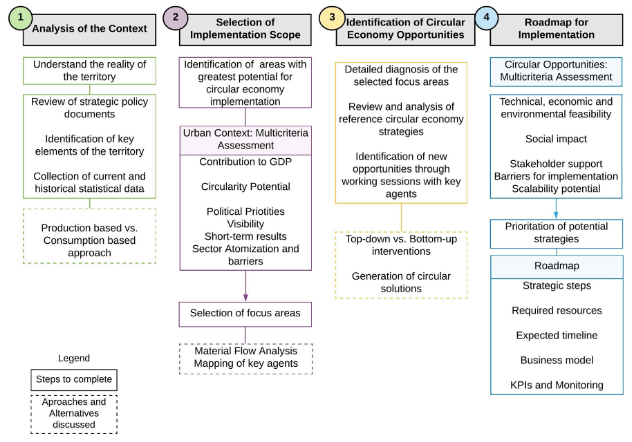
\includegraphics[width=0.8\textwidth]{sections/asset/ce_in_cities.PNG}
    \caption{Methodological proposition to apply CE in cities}
    \label{fig:ce_application}
\end{figure}


\parencite{Korhonen2018a}
Circular economy (CE) is a concept currently promoted by the EU, by several national governments including China, Japan, UK, France, Canada, The Netherlands, Sweden and Finland as well as by several businesses around the world. The European Commission recently esti- mated that circular economy-type economic transitions can create 600 billion euros annual economic gains for the EU manufacturing sector alone (COM, 2014; EMAF, 2013;see also CIRAIG, 2015 and COM, 2015). Finland's Independence Celebration Fund (FICF, SITRA) and Mckinsey (2014) jointly estimate 2.5 billion euros annual gains for the national economy of Finland through circular economy. The global economy would benefit 1000 billion US dollars annually (FICF and Mckinsey, 2014;see e.g. EMAF, 2013). China, as the first country in the world, adopted a law for the circular economy in 2008 (CIRAIG, 2015). Circular economy is recommended as an approach to economic growth that is in line with sustainable environmental and economic develop- ment (see EMAF et al., 2015; EMAF, 2013; EMAF, 2012; CIRAIG, 2015; COM, 2015; COM, 2014).


The scientific and research basis of the CE approach seems to be only in its infancy. To authors' knowledge the definition given above in section three (3) is the first attempt to present a scientific research-based definition of CE. Many key questions are still open. These will arise, e.g. from the nature of self-organized complex social-ecological systems (see e.g., Chertowand Ehrenfeld, 2012; Folke, 2006) to which CE systems belong.


\begin{figure}[h!]
    \centering
    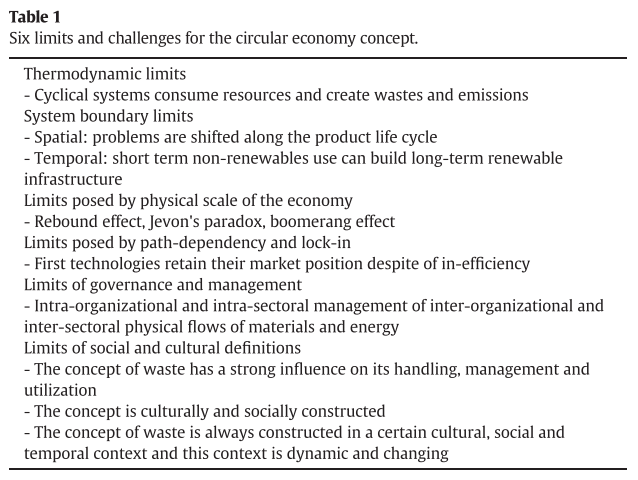
\includegraphics[width=0.8\textwidth]{sections/asset/limits.PNG}
    \caption{Six limits of the concept of CE}
    \label{fig:ce_limits}
\end{figure}


\parencite{Stahel2013}


To overcome this general lack of knowledge, Stahel (2013) outlines a set of principles that would apply in a Circular Economy: (a) the smaller the resource circulation (activity-wise and geographically) the more profitable and resource efficient; (b) material loops are continuous, therefore, materials constantly circulate in the economy and feed into new production processes, minimising potential waste; (c) maintaining the value, quality and performance of goods; (d) the efficiency of managing stocks in CE increases with a decreasing flow speed; (e) extending ownership is a cost-efficient strategy, as reuse, repair and remanufacturing without ownership changes saves on transaction costs; and (f) CE requires the existence of well-functioning second hand product and secondary materials markets. Skene (2017) presents a similar set of principles, and complements further with (g) elimination of toxic substances and (h) renewable energy use.



\parencite{Milios2018}
From a sustainability point of view, CE has been found to lack on considerations towards the social dimension (Broto et al. 2012; Jiao and Boons 2014; Murray et al. 2017). However, Murray et al. (2017) identified that some elements of relevance do exist in the CE narrative, referring to the maximisation of ecosystem functioning and human well-being, apart from the obvious tenet of job creation (locally). Moreover, the strong ‘‘material’’ focus in the current narrative of CE seems to preclude wider systemic considerations of sectoral approaches to CE (Haupt et al. 2017). 

\begin{figure}[h!]
    \centering
    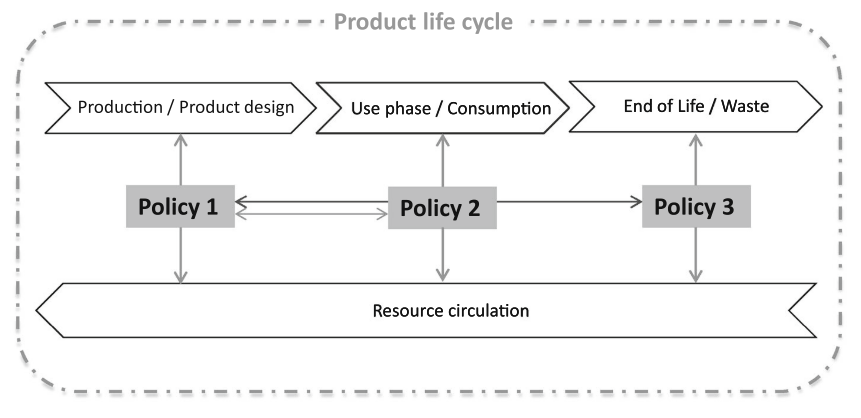
\includegraphics[width=0.8\textwidth]{sections/asset/policies.PNG}
    \caption{Product life cycle and policies}
    \label{fig:ce_policies}
\end{figure}


Nicolli et al. (2012) point out that there is a significant risk of high search and transaction costs associated with recyclable materials in secondary markets, related to incomplete information. There is usually a lack of information concerning the quality and properties of potentially recyclable or reusable materials and products. In addition to this, the provided information is usually asymmetric, in the sense that the supplier holds a negotiating advantage by knowing more about the quality or properties of the material or product than the potential buyer. In such cases, a broad range of policy instruments can be used to support the markets. The establishment of harmonised quality standards for recycled materials and/or certification schemes could be useful in overcoming such barriers (Finnveden et al. 2013)



about measuring Indicators
\parencite{Geng2012}

\begin{figure}[h!]
    \centering
    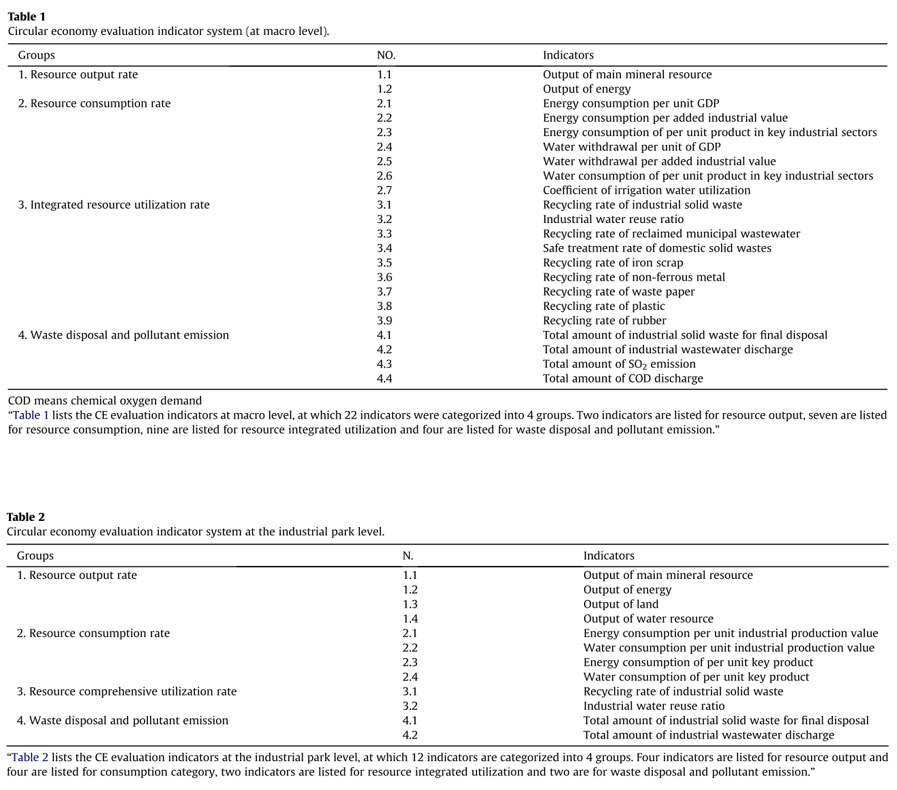
\includegraphics[width=0.8\textwidth]{sections/asset/ce_china_indicators.PNG}
    \caption{Circular Economy indicators in China}
    \label{fig:ce_chinaindi}
\end{figure}



\parencite{eliaMeasuringCircularEconomy2017}
critical of chines indicators


\subsection{Barriers to Circular Economy}


\parencite{Kirchherr2018}

We present the first large-N-study on circular economy barriers in the EU (208 survey respondents, 47 expert interviews). We find that cultural barriers, particularly a lack of consumer interest and awareness as well as a hesitant company culture, are considered the main circular economy barriers by businesses and policy-makers. These are driven by market barriers which, in turn, are induced by a lack of synergistic governmental interventions to accelerate the transition towards a circular economy. Meanwhile, not a single technological barrier is ranked among the most pressing circular economy barriers, according to our research. Overall, our work suggests that circular economy is a niche discussion among sustainable development professionals at this stage. Significant efforts need to be undertaken for the concept to maintain its momentum. \par

\begin{figure}[h!]
    \centering
    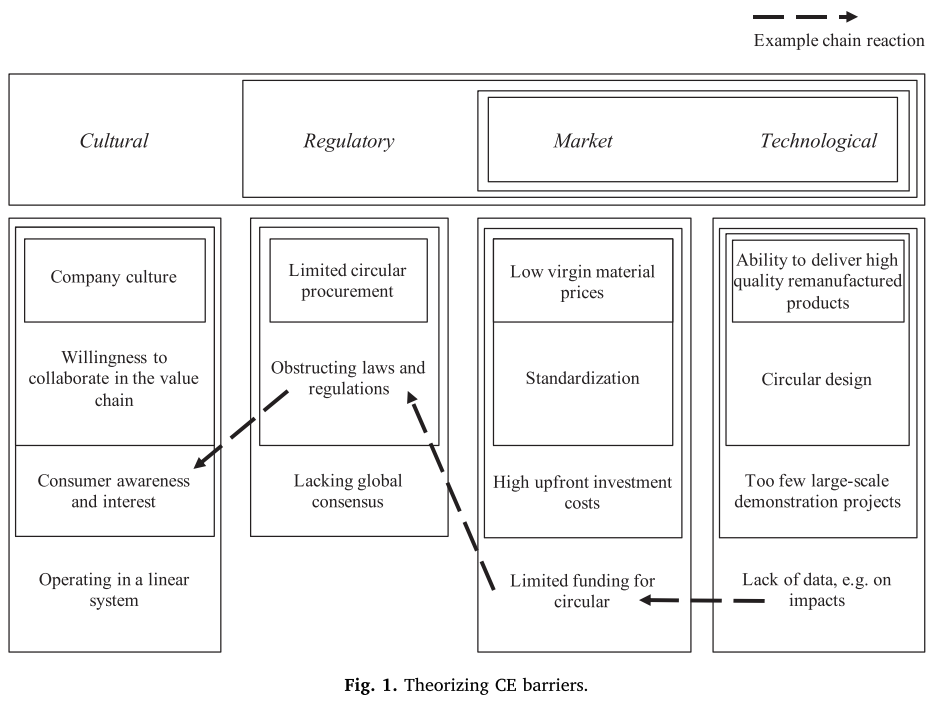
\includegraphics[width=0.8\textwidth]{sections/asset/barriers.PNG}
    \caption{Barriers to implement CE}
    \label{fig:ce_BARRIERS}
\end{figure}

\begin{figure}[h!]
    \centering
    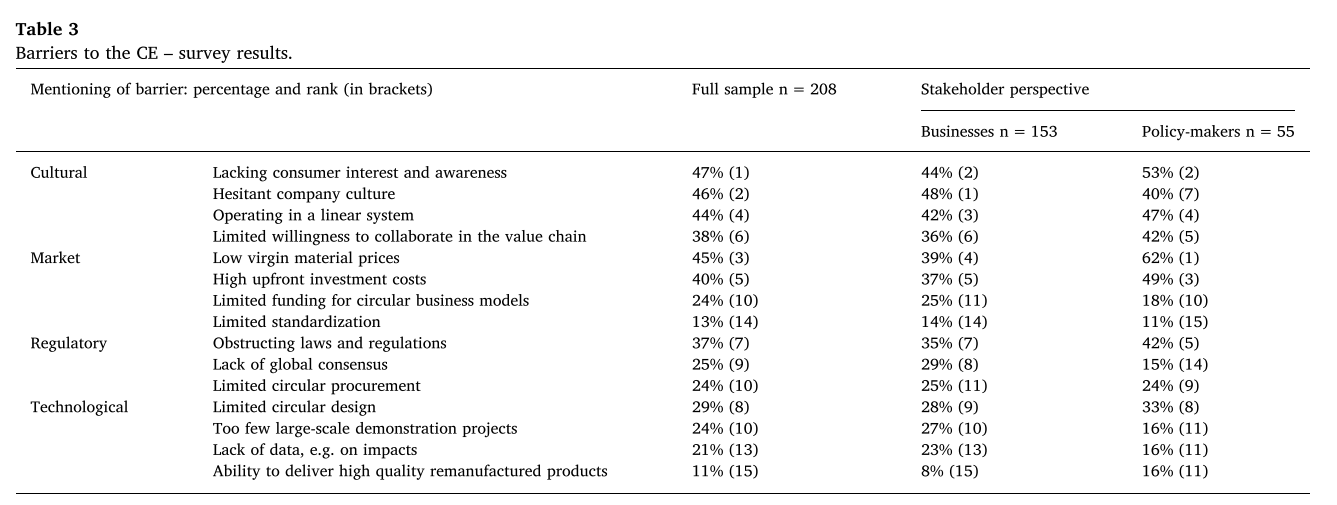
\includegraphics[width=0.8\textwidth]{sections/asset/BARRIER_SPECS.PNG}
    \caption{Survey results}
    \label{fig:ce_BARRIERS}
\end{figure}

The CE concept is gaining momentum these days as an allegedly
novel pathway towards sustainable development. Particularly the EU has endorsed the concept. Despite the growing attention and endorsement received, the CE has seen limited implementation so far. Those writing on the CE frequently blame the limited CE implementation on various barriers, with technological barriers having emerged in the literature as the alleged core barriers that impede the transition towards a CE. \par


\parencite{Shahbazi2016}
\begin{figure}[h!]
    \centering
    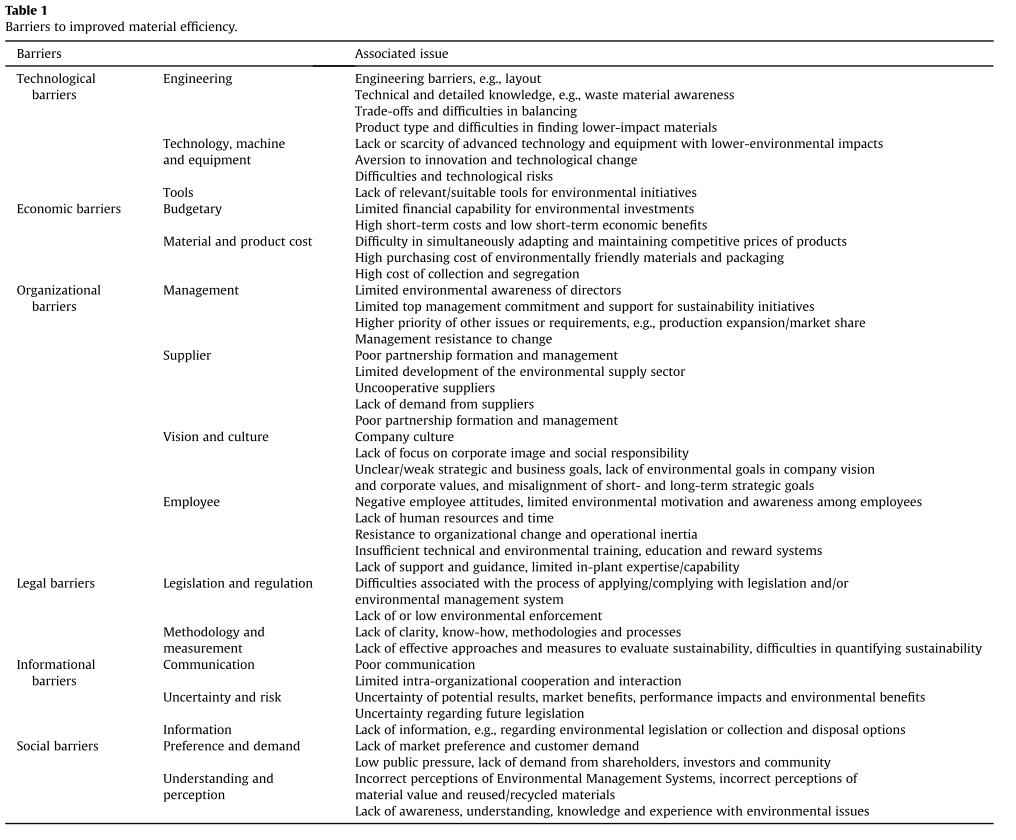
\includegraphics[width=0.8\textwidth]{sections/asset/more_barriers.PNG}
    \caption{More barriers to improve resource efficiency}
    \label{fig:ce_BARRIERS1}
\end{figure}


\parencite{Ritzen2017}
These barriers relate to what CE is – barriers for closing material loops, delivering new offers to customers, making requirements and expectations of suppliers and on customers, and developing the whole supply chain. Also, how their current businesses are conducted is strongly connected to these barriers. When analyzing the case companies in greater detail, we also see barriers rather related to the actual transition towards CE, and they tend clearly to concern integration of different perspectives and of different domains. These barriers are in several ways similar to barriers to integration of environmental aspects, though is likely challenges of larger altitudes as they encompass every function and every level in the organization and take sustainability issues to a strategic level. These working way that is needed for performing the required disruptive changes and radical innovations. \par


Finally, as an integration barrier we see the lack of
integration throughout the supply chain, also identified among respondents. Possible solutions for closing material loops are requiring a closer connection between suppliers and producers and between producer and customers. The characteristics of these two different companies matter for which barriers are revealed, in relation to their business logic.However, what they have in common is that also for disruptive changes more collaboration is necessary for innovation in the eco-systems of different actors [37, 38]\par

In addition to integration barriers, the barrier connected to knowledge and an exploratory way of working needs to be addressed.
Knowledge is not only of concern for its content, with lack of knowledge as a barrier, but also for how companies regard knowledge creation and how this is managed within innovation. The ability to perform radical innovations is strongly connected to an explorative way of working, deeply connected to how knowledge is gained. In exploration, knowledge is looked for outside the company, and experiments are made for learning purposes in invention activities [24].\par


\parencite{Ritzen2017}

\subsubsection{Overcoming challenges}
\parencite{Bressanelli2018}

\parencite{Okorie}

\subsection{Circular Flow of resources}








\subsubsection{Industrial Symbiosis}



\parencite{Almeida2015}
strategies for cleaner production
\begin{figure}[h!]
    \centering
    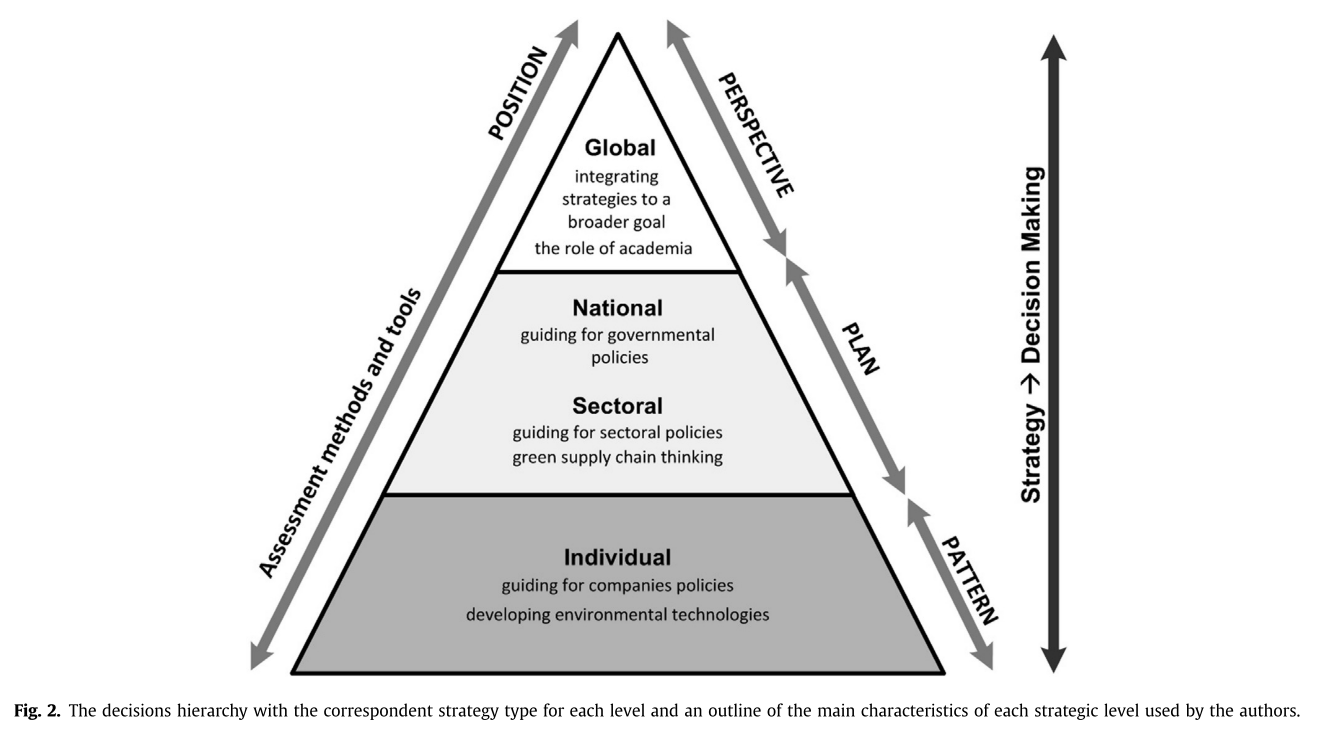
\includegraphics[width=0.8\textwidth]{sections/asset/clean production.PNG}
    \caption{Clean production strategies}
    \label{fig:cp_stategies}
\end{figure}

{Industry 4.0}



\subsubsection{Waste}
\parencite{OakdeneHollins2017} - Towards a circular economy - waste mgmt in the eu

{Industry 4.0}
\parencite{Vafeiadis2019}








